% Options for packages loaded elsewhere
% Options for packages loaded elsewhere
\PassOptionsToPackage{unicode}{hyperref}
\PassOptionsToPackage{hyphens}{url}
\PassOptionsToPackage{dvipsnames,svgnames,x11names}{xcolor}
%
\documentclass[
  11pt,
  letterpaper,
  DIV=11,
  numbers=noendperiod]{scrartcl}
\usepackage{xcolor}
\usepackage[margin=2.5cm]{geometry}
\usepackage{amsmath,amssymb}
\setcounter{secnumdepth}{5}
\usepackage{iftex}
\ifPDFTeX
  \usepackage[T1]{fontenc}
  \usepackage[utf8]{inputenc}
  \usepackage{textcomp} % provide euro and other symbols
\else % if luatex or xetex
  \usepackage{unicode-math} % this also loads fontspec
  \defaultfontfeatures{Scale=MatchLowercase}
  \defaultfontfeatures[\rmfamily]{Ligatures=TeX,Scale=1}
\fi
\usepackage{lmodern}
\ifPDFTeX\else
  % xetex/luatex font selection
\fi
% Use upquote if available, for straight quotes in verbatim environments
\IfFileExists{upquote.sty}{\usepackage{upquote}}{}
\IfFileExists{microtype.sty}{% use microtype if available
  \usepackage[]{microtype}
  \UseMicrotypeSet[protrusion]{basicmath} % disable protrusion for tt fonts
}{}
\makeatletter
\@ifundefined{KOMAClassName}{% if non-KOMA class
  \IfFileExists{parskip.sty}{%
    \usepackage{parskip}
  }{% else
    \setlength{\parindent}{0pt}
    \setlength{\parskip}{6pt plus 2pt minus 1pt}}
}{% if KOMA class
  \KOMAoptions{parskip=half}}
\makeatother
% Make \paragraph and \subparagraph free-standing
\makeatletter
\ifx\paragraph\undefined\else
  \let\oldparagraph\paragraph
  \renewcommand{\paragraph}{
    \@ifstar
      \xxxParagraphStar
      \xxxParagraphNoStar
  }
  \newcommand{\xxxParagraphStar}[1]{\oldparagraph*{#1}\mbox{}}
  \newcommand{\xxxParagraphNoStar}[1]{\oldparagraph{#1}\mbox{}}
\fi
\ifx\subparagraph\undefined\else
  \let\oldsubparagraph\subparagraph
  \renewcommand{\subparagraph}{
    \@ifstar
      \xxxSubParagraphStar
      \xxxSubParagraphNoStar
  }
  \newcommand{\xxxSubParagraphStar}[1]{\oldsubparagraph*{#1}\mbox{}}
  \newcommand{\xxxSubParagraphNoStar}[1]{\oldsubparagraph{#1}\mbox{}}
\fi
\makeatother


\usepackage{longtable,booktabs,array}
\usepackage{calc} % for calculating minipage widths
% Correct order of tables after \paragraph or \subparagraph
\usepackage{etoolbox}
\makeatletter
\patchcmd\longtable{\par}{\if@noskipsec\mbox{}\fi\par}{}{}
\makeatother
% Allow footnotes in longtable head/foot
\IfFileExists{footnotehyper.sty}{\usepackage{footnotehyper}}{\usepackage{footnote}}
\makesavenoteenv{longtable}
\usepackage{graphicx}
\makeatletter
\newsavebox\pandoc@box
\newcommand*\pandocbounded[1]{% scales image to fit in text height/width
  \sbox\pandoc@box{#1}%
  \Gscale@div\@tempa{\textheight}{\dimexpr\ht\pandoc@box+\dp\pandoc@box\relax}%
  \Gscale@div\@tempb{\linewidth}{\wd\pandoc@box}%
  \ifdim\@tempb\p@<\@tempa\p@\let\@tempa\@tempb\fi% select the smaller of both
  \ifdim\@tempa\p@<\p@\scalebox{\@tempa}{\usebox\pandoc@box}%
  \else\usebox{\pandoc@box}%
  \fi%
}
% Set default figure placement to htbp
\def\fps@figure{htbp}
\makeatother





\setlength{\emergencystretch}{3em} % prevent overfull lines

\providecommand{\tightlist}{%
  \setlength{\itemsep}{0pt}\setlength{\parskip}{0pt}}



 


\KOMAoption{captions}{tableheading}
\makeatletter
\@ifpackageloaded{caption}{}{\usepackage{caption}}
\AtBeginDocument{%
\ifdefined\contentsname
  \renewcommand*\contentsname{Table of contents}
\else
  \newcommand\contentsname{Table of contents}
\fi
\ifdefined\listfigurename
  \renewcommand*\listfigurename{List of Figures}
\else
  \newcommand\listfigurename{List of Figures}
\fi
\ifdefined\listtablename
  \renewcommand*\listtablename{List of Tables}
\else
  \newcommand\listtablename{List of Tables}
\fi
\ifdefined\figurename
  \renewcommand*\figurename{Figure}
\else
  \newcommand\figurename{Figure}
\fi
\ifdefined\tablename
  \renewcommand*\tablename{Table}
\else
  \newcommand\tablename{Table}
\fi
}
\@ifpackageloaded{float}{}{\usepackage{float}}
\floatstyle{ruled}
\@ifundefined{c@chapter}{\newfloat{codelisting}{h}{lop}}{\newfloat{codelisting}{h}{lop}[chapter]}
\floatname{codelisting}{Listing}
\newcommand*\listoflistings{\listof{codelisting}{List of Listings}}
\makeatother
\makeatletter
\makeatother
\makeatletter
\@ifpackageloaded{caption}{}{\usepackage{caption}}
\@ifpackageloaded{subcaption}{}{\usepackage{subcaption}}
\makeatother
\usepackage{bookmark}
\IfFileExists{xurl.sty}{\usepackage{xurl}}{} % add URL line breaks if available
\urlstyle{same}
\hypersetup{
  pdftitle={Fengping River Hydropower --- Main Analysis},
  pdfauthor={{[}MAYA SCANLON , WILLIAM LIEN{]}},
  colorlinks=true,
  linkcolor={blue},
  filecolor={Maroon},
  citecolor={Blue},
  urlcolor={Blue},
  pdfcreator={LaTeX via pandoc}}


\title{Fengping River Hydropower --- Main Analysis}
\usepackage{etoolbox}
\makeatletter
\providecommand{\subtitle}[1]{% add subtitle to \maketitle
  \apptocmd{\@title}{\par {\large #1 \par}}{}{}
}
\makeatother
\subtitle{Financial Feasibility Frontier under Hydrological Variability}
\author{{[}MAYA SCANLON , WILLIAM LIEN{]}}
\date{2026-06-03}
\begin{document}
\maketitle

\renewcommand*\contentsname{Table of contents}
{
\hypersetup{linkcolor=}
\setcounter{tocdepth}{2}
\tableofcontents
}

\section{Sediment and Rating Curve}\label{sediment-and-rating-curve}

\subsection{Suspended Sediment Rating
Curve}\label{suspended-sediment-rating-curve}

The suspended sediment load (SSL, MT/day) is estimated from daily
discharge \(Q\) (cms) via a power-law rating curve calibrated on 492
field observations (1959--2023):

\[SSL = a \cdot Q^b\]

fitted by ordinary least squares in log-log space. Only observations
flagged \texttt{ok} with detectable sediment concentration are used;
below-detection-limit records are excluded.

\begin{figure}[H]

{\centering \pandocbounded{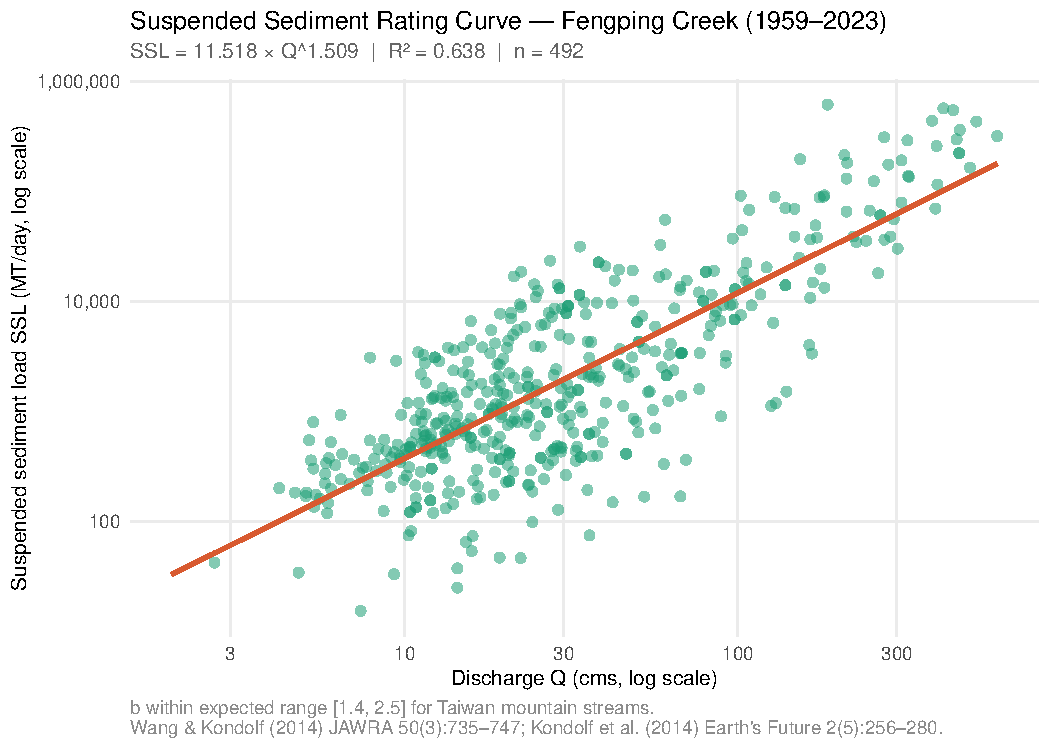
\includegraphics[keepaspectratio]{fp_hydro_main_files/figure-pdf/rating-curve-1.pdf}}

}

\caption{Suspended sediment rating curve for Fengping Creek. Each point
is one field sampling event (n = 492, flag == `ok'). The exponent b =
1.51 falls within the range {[}1.4, 2.5{]} documented for Taiwan
mountain streams (Wang \& Kondolf 2014; Kondolf et al.~2014).}

\end{figure}%

\subsection{Reservoir Sedimentation --- W1 and
W2}\label{reservoir-sedimentation-w1-and-w2}

Trap efficiency \(TE\) is computed annually using the Brune (1953)
curve:

\[TE_t = \frac{CI_t}{CI_t + 0.0021}, \quad CI_t = \frac{S_t}{V_{\text{annual}}}\]

where \(S_t\) is the remaining effective storage (m³) and
\(V_{\text{annual}}\) is the mean annual inflow volume.

\begin{figure}[H]

{\centering \pandocbounded{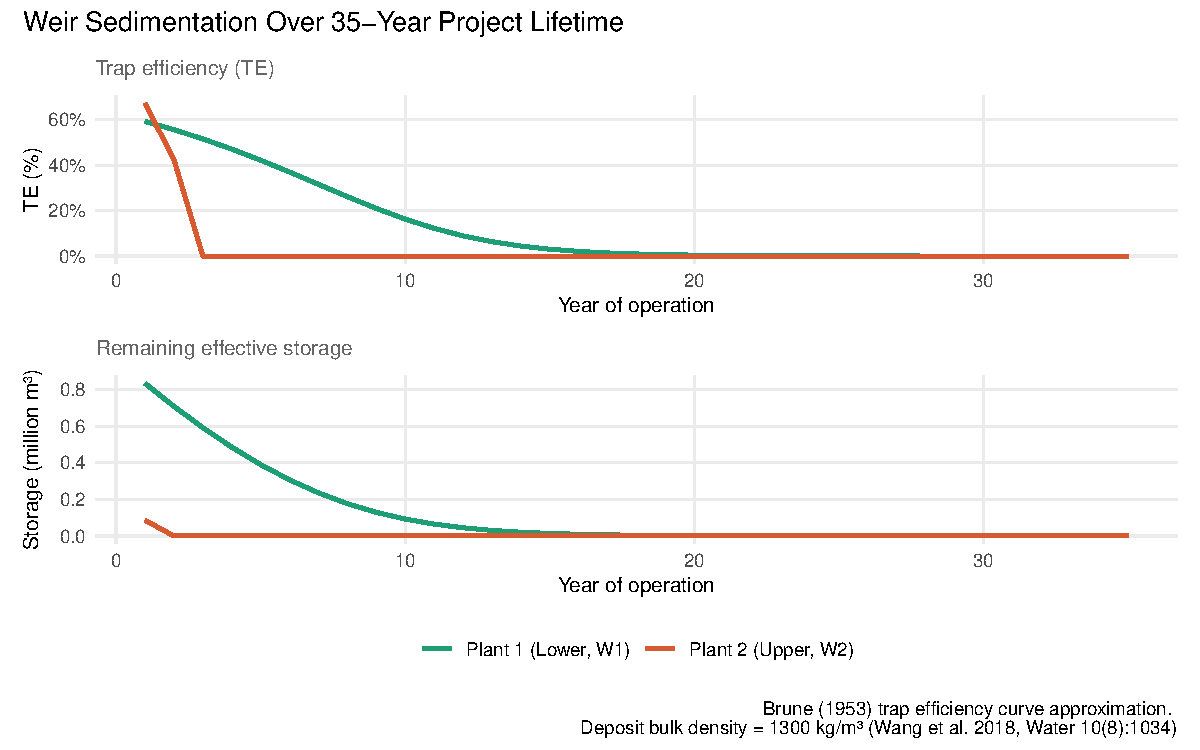
\includegraphics[keepaspectratio]{fp_hydro_main_files/figure-pdf/trap-plot-1.pdf}}

}

\caption{Simulated trap efficiency (TE) and remaining effective storage
for W1 and W2 over the 35-year project lifetime. Brune (1953) curve
approximation; deposit bulk density = 1300 kg/m³ (Wang et al.~2018).}

\end{figure}%

\begin{longtable}[]{@{}lrrrr@{}}
\caption{Trap efficiency and remaining effective storage at key project
milestones (years 1, 10, 20, 35).}\tabularnewline
\toprule\noalign{}
Weir & Year & S remaining (m³) & TE & V loss (m³/yr) \\
\midrule\noalign{}
\endfirsthead
\toprule\noalign{}
Weir & Year & S remaining (m³) & TE & V loss (m³/yr) \\
\midrule\noalign{}
\endhead
\bottomrule\noalign{}
\endlastfoot
W1 Lower & 1 & 0 & 0.375 & 5,765,603 \\
W1 Lower & 10 & 0 & 0.000 & 0 \\
W1 Lower & 20 & 0 & 0.000 & 0 \\
W1 Lower & 35 & 0 & 0.000 & 0 \\
W2 Upper & 1 & 0 & 0.363 & 5,567,670 \\
W2 Upper & 10 & 0 & 0.000 & 0 \\
W2 Upper & 20 & 0 & 0.000 & 0 \\
W2 Upper & 35 & 0 & 0.000 & 0 \\
\end{longtable}

\begin{center}\rule{0.5\linewidth}{0.5pt}\end{center}

\section{Reservoir Simulation --- Historical
Baseline}\label{reservoir-simulation-historical-baseline}

The pondage simulation (\texttt{simulate\_one\_weir()}) uses a daily
Euler forward water balance with a strict dispatch priority: (1)
ecological flow, (2) power generation up to \(Q_{\text{design}}\), (3)
spillage.

The 24-hour forecast model (\texttt{simulate\_one\_weir\_forward24()})
additionally looks ahead one day to decide how much water to retain,
reducing spill during high-flow events while smoothing generation during
droughts.

Both models are run on the full historical record (1958--2025) with the
\textbf{recommended ecological flow} (W1 = 5.0 cms, W2 = 1.0 cms).

\subsection{Operation Window --- Interactive Date
Selection}\label{operation-window-interactive-date-selection}

Change \texttt{START\_DATE} and \texttt{END\_DATE} to inspect any period
of interest.

\begin{figure}[H]

{\centering \pandocbounded{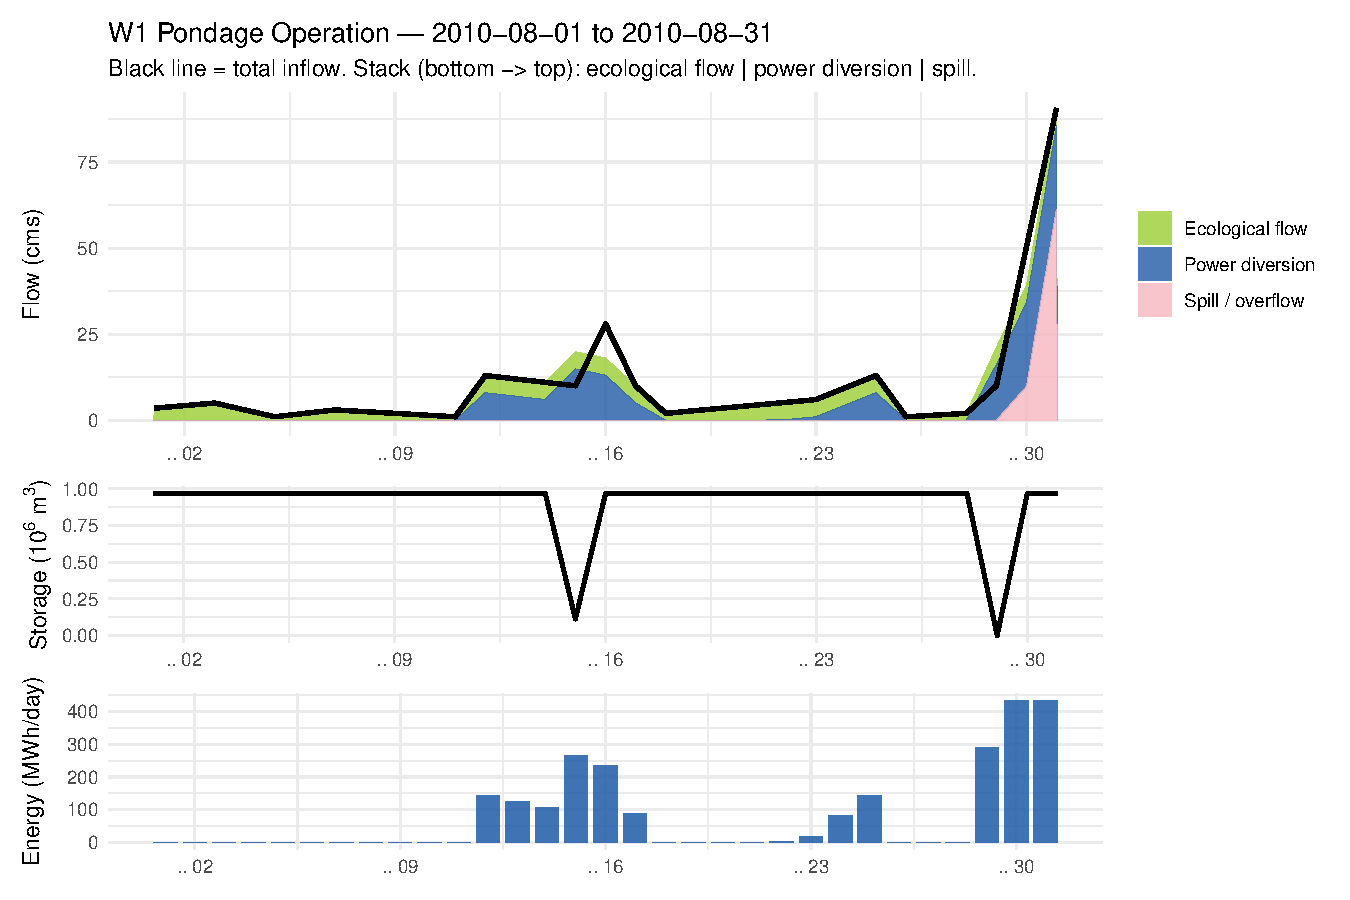
\includegraphics[keepaspectratio]{fp_hydro_main_files/figure-pdf/operation-window-1.pdf}}

}

\caption{W1 reservoir operation during a representative typhoon-season
window. Line = inflow; stacked areas = ecological flow, power diversion,
and spill. Lower panels show storage trajectory and daily energy.}

\end{figure}%

\subsection{Annual Energy --- Calendar
Heatmap}\label{annual-energy-calendar-heatmap}

\begin{figure}[H]

{\centering \pandocbounded{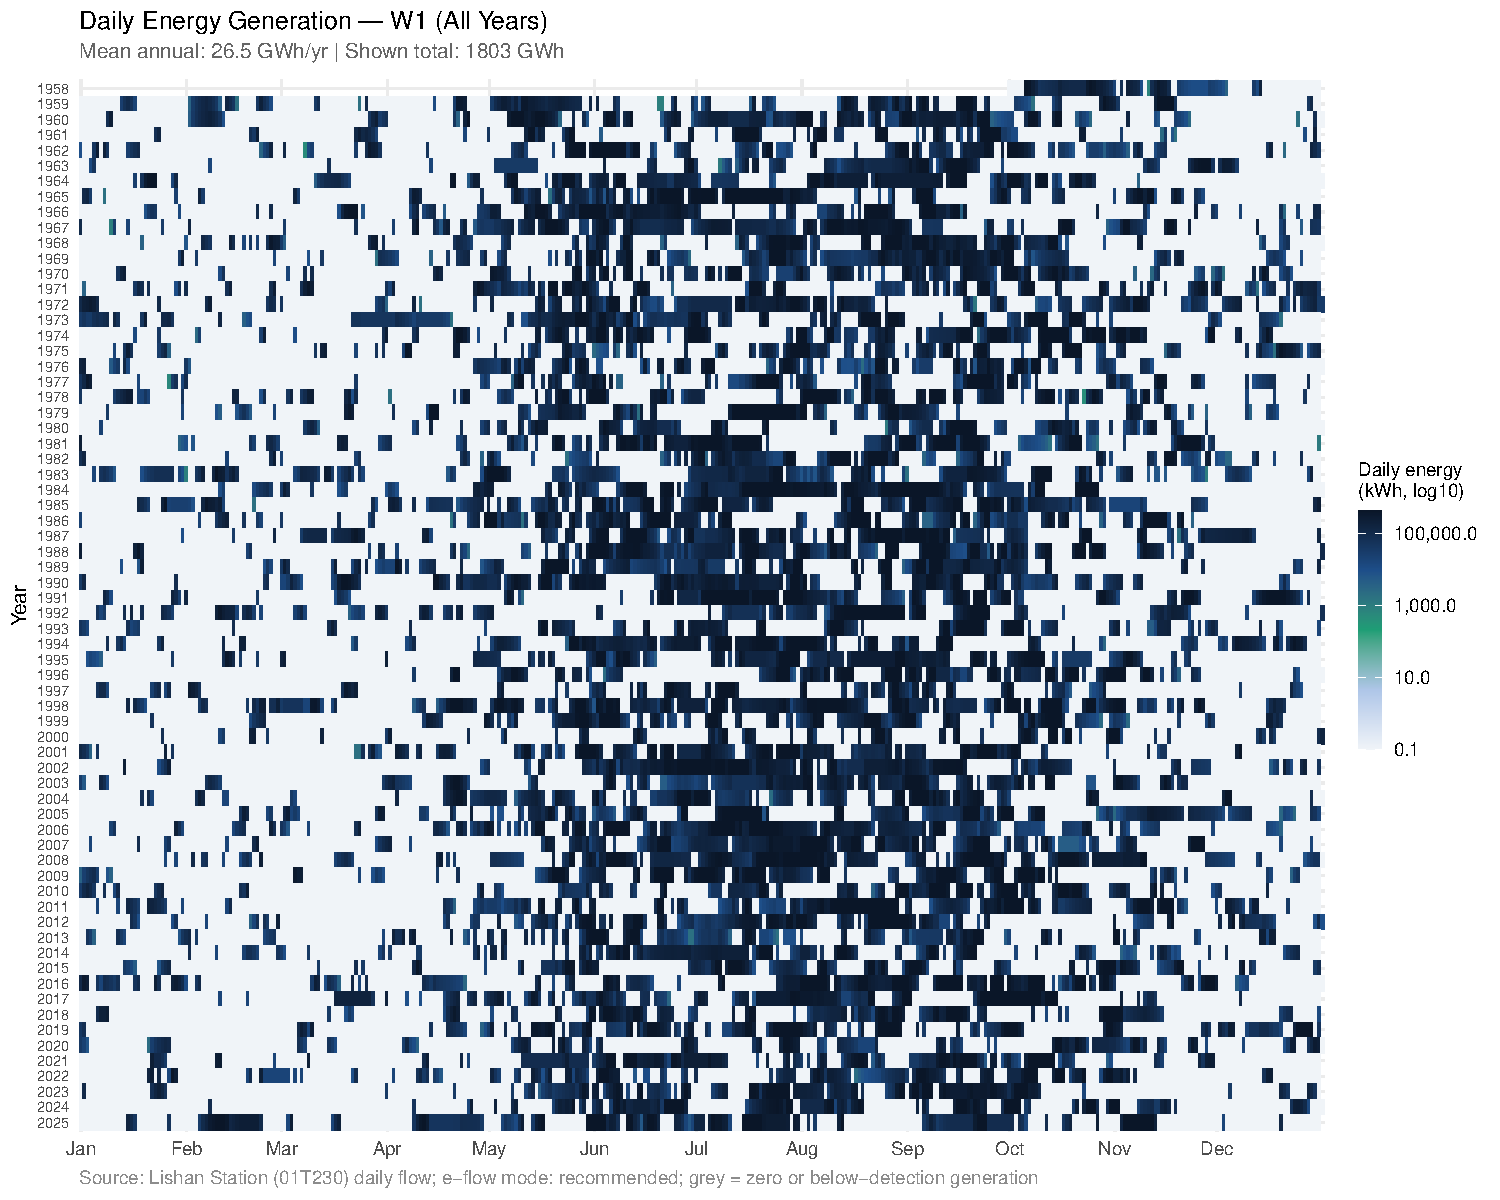
\includegraphics[keepaspectratio]{fp_hydro_main_files/figure-pdf/heatmap-1.pdf}}

}

\caption{Calendar heatmap of daily energy generation for W1 (pondage
mode, 1958--2025). Dark = high generation; grey = near-zero.
Typhoon-season pulses visible as dark horizontal bands in
July--September.}

\end{figure}%

\subsection{Annual Generation Summary --- Run-of-River vs
Pondage}\label{annual-generation-summary-run-of-river-vs-pondage}

\begin{longtable}[]{@{}
  >{\raggedright\arraybackslash}p{(\linewidth - 8\tabcolsep) * \real{0.2162}}
  >{\raggedleft\arraybackslash}p{(\linewidth - 8\tabcolsep) * \real{0.1622}}
  >{\raggedleft\arraybackslash}p{(\linewidth - 8\tabcolsep) * \real{0.1486}}
  >{\raggedleft\arraybackslash}p{(\linewidth - 8\tabcolsep) * \real{0.1486}}
  >{\raggedleft\arraybackslash}p{(\linewidth - 8\tabcolsep) * \real{0.3243}}@{}}
\caption{Annual generation statistics for W1 + W2 combined. Revenue
computed at PPA rate (NTD 6.0/kWh). Run-of-river = immediate dispatch;
Pondage = 24-hour forecast-informed. Historical record
1958--2025.}\tabularnewline
\toprule\noalign{}
\begin{minipage}[b]{\linewidth}\raggedright
Mode
\end{minipage} & \begin{minipage}[b]{\linewidth}\raggedleft
Mean GWh/yr
\end{minipage} & \begin{minipage}[b]{\linewidth}\raggedleft
P10 GWh/yr
\end{minipage} & \begin{minipage}[b]{\linewidth}\raggedleft
P90 GWh/yr
\end{minipage} & \begin{minipage}[b]{\linewidth}\raggedleft
Mean Revenue (NTD B/yr)
\end{minipage} \\
\midrule\noalign{}
\endfirsthead
\toprule\noalign{}
\begin{minipage}[b]{\linewidth}\raggedright
Mode
\end{minipage} & \begin{minipage}[b]{\linewidth}\raggedleft
Mean GWh/yr
\end{minipage} & \begin{minipage}[b]{\linewidth}\raggedleft
P10 GWh/yr
\end{minipage} & \begin{minipage}[b]{\linewidth}\raggedleft
P90 GWh/yr
\end{minipage} & \begin{minipage}[b]{\linewidth}\raggedleft
Mean Revenue (NTD B/yr)
\end{minipage} \\
\midrule\noalign{}
\endhead
\bottomrule\noalign{}
\endlastfoot
Run-of-river & 45.2 & 29 & 58 & 0.271 \\
Pondage (24-hr) & 48.2 & 31 & 62 & 0.289 \\
\end{longtable}

\begin{center}\rule{0.5\linewidth}{0.5pt}\end{center}

\section{35-Year NPV Trajectory --- Historical
Baseline}\label{year-npv-trajectory-historical-baseline}

NPV is computed using equity discount rate \(r_e = 8\%\), LTV = 80\%,
and loan rate \(r_{\ell} = 3\%\). Electricity revenue uses the PPA rate
(NTD 6/kWh). Three CAPEX scenarios are compared:

\begin{itemize}
\tightlist
\item
  \textbf{CAPEX\textsubscript{OG}} = NTD 5.0 billion (earliest public
  announcement)
\item
  \textbf{CAPEX\textsubscript{EIA}} = NTD 6.4 billion (1999 EIA
  feasibility report)
\item
  \textbf{CAPEX\textsubscript{2025}} = NTD 9.7 billion (2025 investor
  conference)
\end{itemize}

\begin{figure}[H]

{\centering \pandocbounded{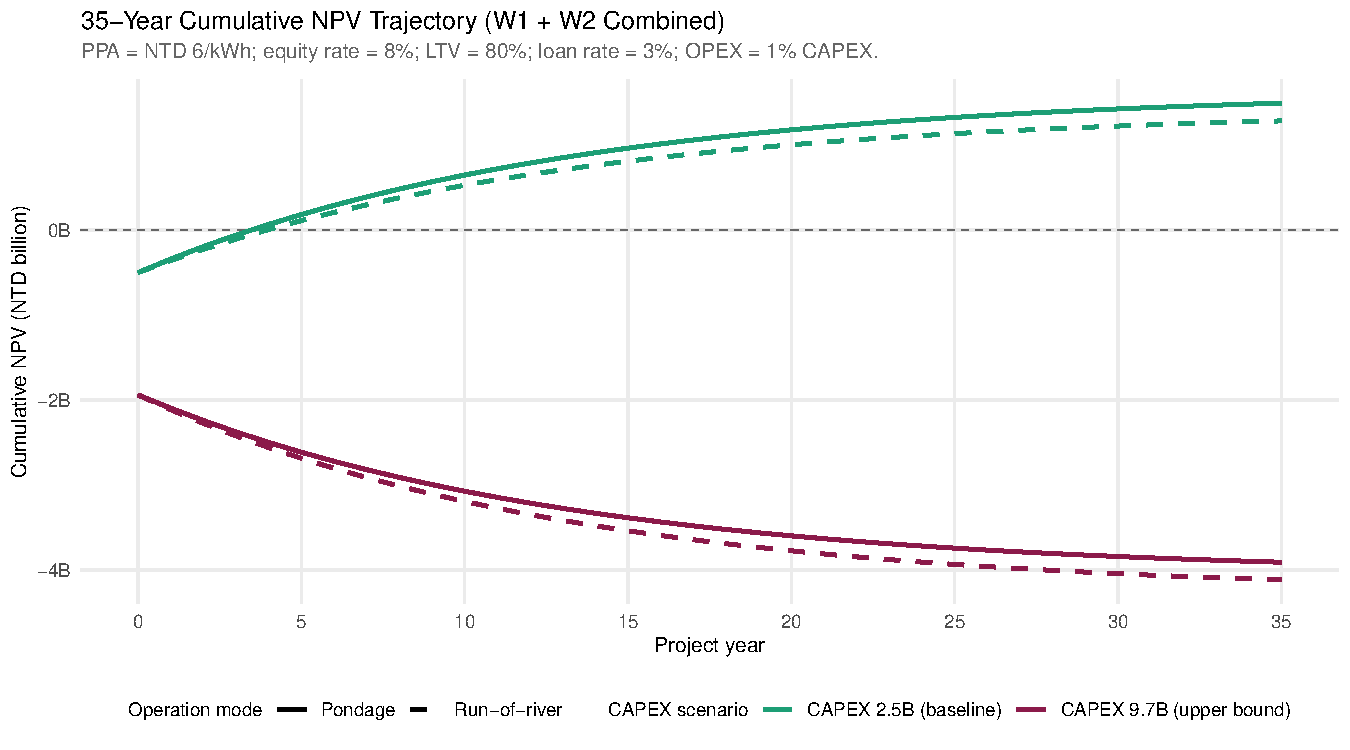
\includegraphics[keepaspectratio]{fp_hydro_main_files/figure-pdf/npv-trajectory-1.pdf}}

}

\caption{35-year cumulative NPV trajectory for both operation modes and
two CAPEX scenarios. Baseline: 25億 NTD (20億 civil + 5億 Tx/E\&M);
Upper bound: 97億 NTD (2025 investor conference). Revenue at PPA rate
(NTD 6.0/kWh). Dashed horizontal line = NPV breakeven.}

\end{figure}%

\begin{center}\rule{0.5\linewidth}{0.5pt}\end{center}

\section{Climate Bootstrap --- Hydrological Variability
Ensemble}\label{climate-bootstrap-hydrological-variability-ensemble}

\subsection{Bootstrap Design}\label{bootstrap-design}

Two-layer bootstrap (Section 3 of \texttt{hydro\_climate.R}):

\begin{enumerate}
\def\labelenumi{\arabic{enumi}.}
\item
  \textbf{Layer 1 --- Whole-year block bootstrap}: draw complete
  calendar years with replacement from the observed record (1958--2025),
  preserving within-year seasonal structure and typhoon event integrity.
\item
  \textbf{Layer 2 --- CV scaling}: rescale daily flows around the annual
  mean to a target within-year CV level:
\end{enumerate}

\[Q_{\text{scaled}}(t) = \mu_{yr} + (Q_{\text{boot}}(t) - \mu_{yr}) \times \lambda, \quad \lambda = \frac{CV_{\text{target}}}{CV_{\text{boot}}}\]

This preserves \(\mu_{yr}\) exactly while enabling CV values beyond the
historical range, consistent with SSP2-4.5 and SSP5-8.5 projections for
eastern Taiwan (Shiau \& Huang 2014; Tung et al.~2016; IPCC AR6 Ch. 11).

\subsection{CV Scaling Validation}\label{cv-scaling-validation}

\begin{figure}[H]

{\centering \pandocbounded{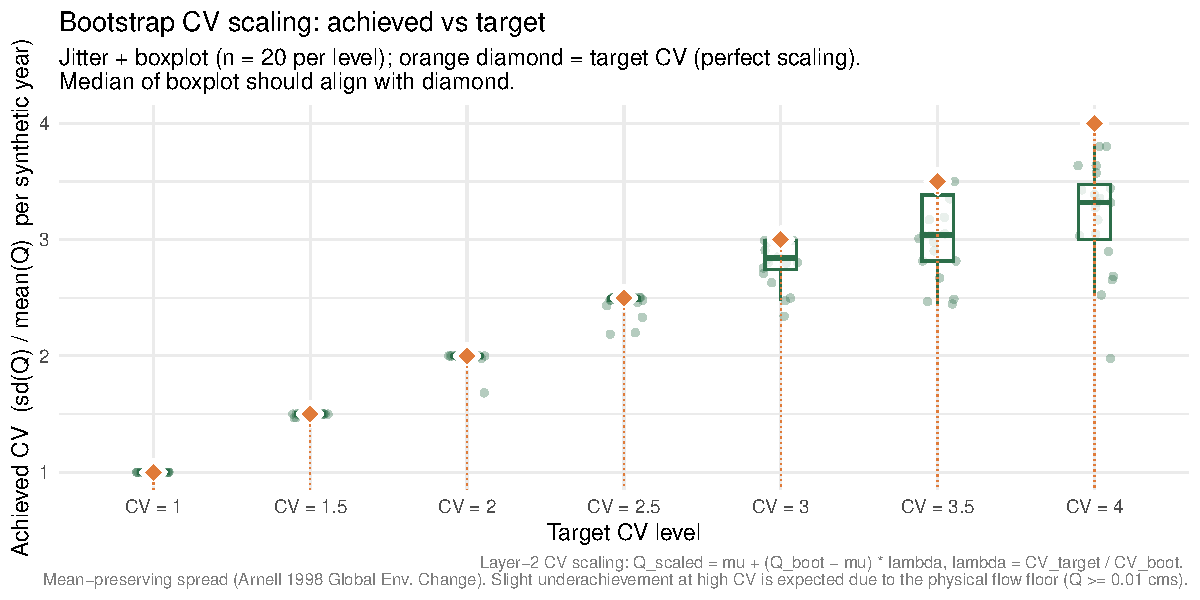
\includegraphics[keepaspectratio]{fp_hydro_main_files/figure-pdf/cv-validation-1.pdf}}

}

\caption{Validation of Layer-2 CV scaling. Violin plots show the
distribution of achieved CV across 200 bootstrap replicates for each
target CV level. Diamonds mark the target. The median should lie close
to each target; slight underestimation at high CV levels is expected due
to the physical flow floor constraint.}

\end{figure}%

\begin{figure}[H]

{\centering \pandocbounded{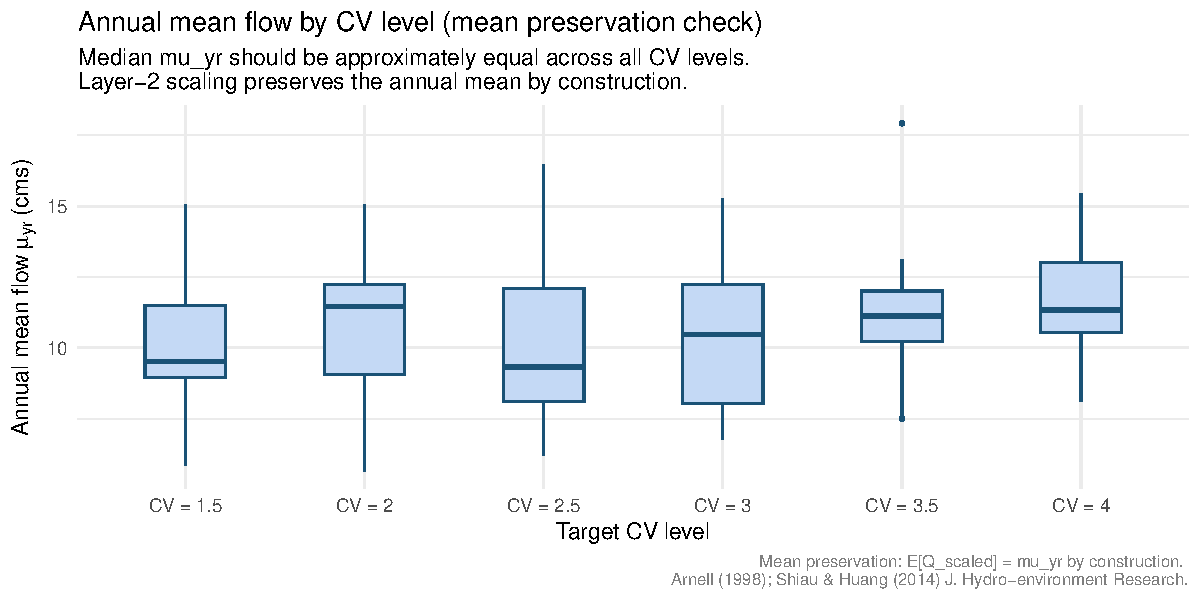
\includegraphics[keepaspectratio]{fp_hydro_main_files/figure-pdf/mu-preservation-1.pdf}}

}

\caption{Mean-preservation check: annual mean flow (mu\_yr) should be
approximately constant across CV levels, confirming that Layer 2 does
not alter the mean --- only the variability.}

\end{figure}%

\subsection{Historical CV Trend}\label{historical-cv-trend}

\begin{figure}[H]

{\centering \pandocbounded{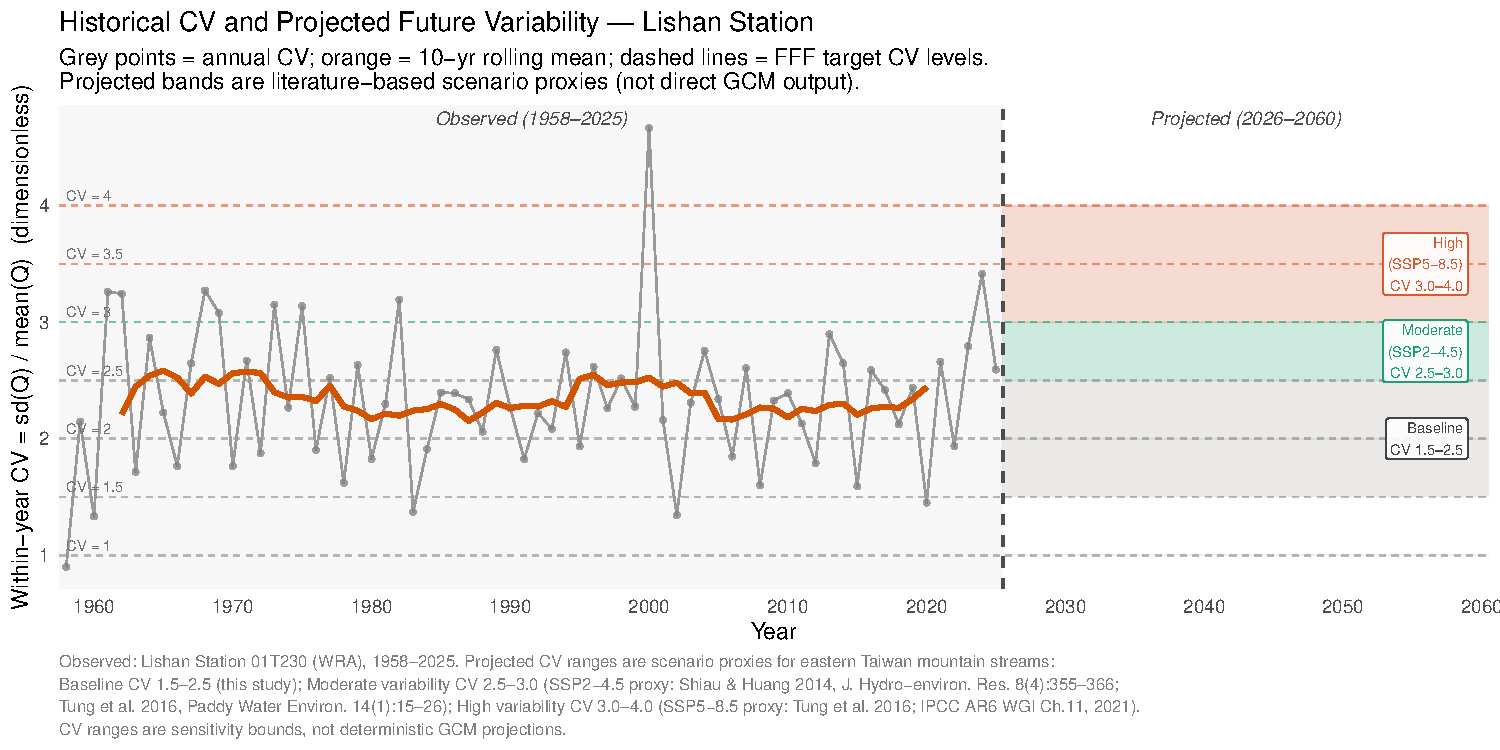
\includegraphics[keepaspectratio]{fp_hydro_main_files/figure-pdf/cv-trend-1.pdf}}

}

\caption{Historical within-year CV (1958--2025) and projected future
variability scenario bands (2026--2060). Left zone: observed annual CV
(grey points) with 10-year rolling mean (orange). Right zone:
literature-based scenario proxies --- Baseline (CV 1.5--2.5),
Moderate/SSP2-4.5 (CV 2.5--3.0), High/SSP5-8.5 (CV 3.0--4.0). Vertical
dashed line separates observed history from projected window. Sources:
Shiau \& Huang (2014); Tung et al.~(2016); IPCC AR6 WGI Ch.11 (2021).}

\end{figure}%

\subsection{Bootstrap CV Distribution --- Option A (target CV on
X-axis)}\label{bootstrap-cv-distribution-option-a-target-cv-on-x-axis}

\begin{figure}[H]

{\centering \pandocbounded{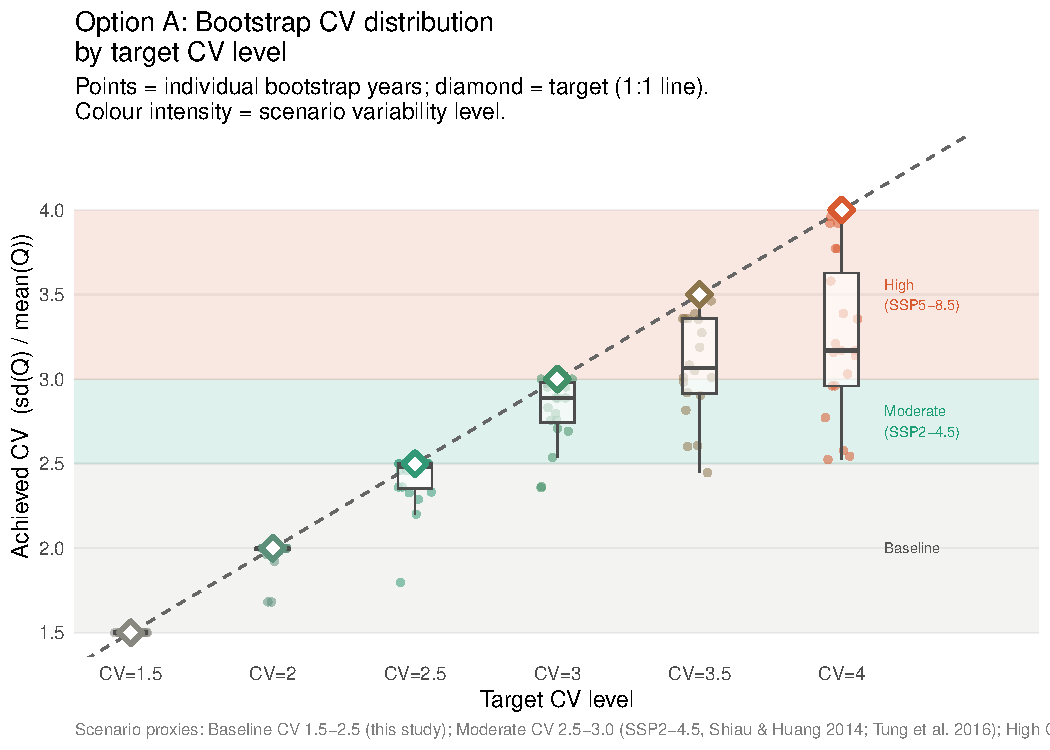
\includegraphics[keepaspectratio]{fp_hydro_main_files/figure-pdf/cv-bootstrap-A-1.pdf}}

}

\caption{Option A: Bootstrap CV scaling validation. X-axis = target CV
level; Y-axis = achieved CV per synthetic year. Each point is one
bootstrap replicate. Diamond = perfect 1:1 target. Background bands show
scenario zones. Median should align with diamond.}

\end{figure}%

\subsection{Bootstrap CV Distribution --- Option B (all simulations
coloured by
level)}\label{bootstrap-cv-distribution-option-b-all-simulations-coloured-by-level}

\begin{figure}[H]

{\centering \pandocbounded{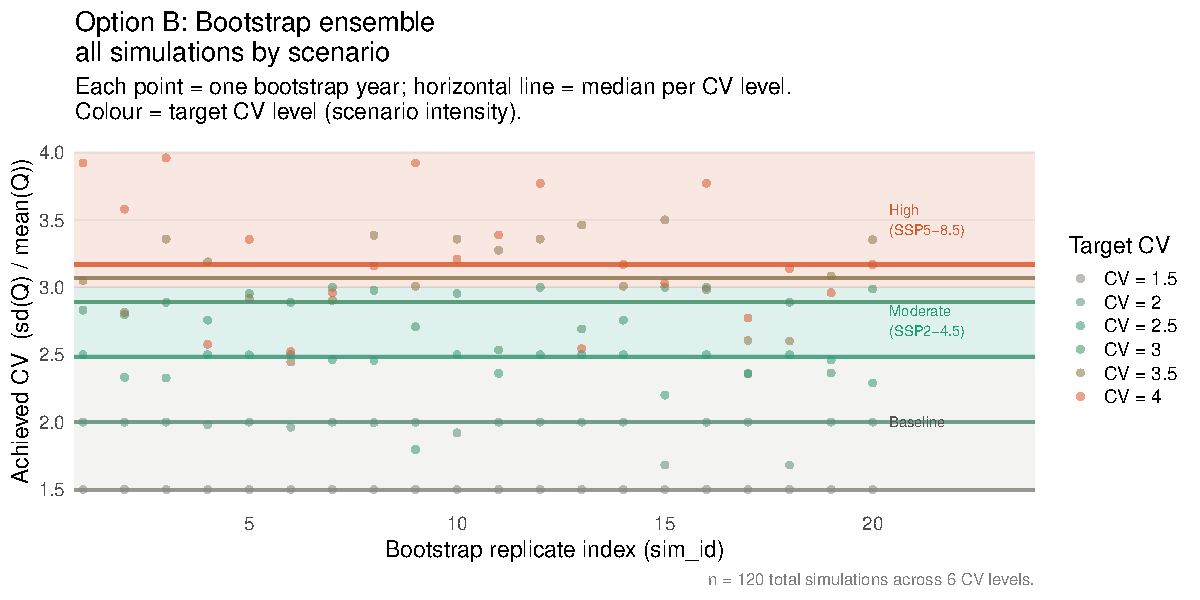
\includegraphics[keepaspectratio]{fp_hydro_main_files/figure-pdf/cv-bootstrap-B-1.pdf}}

}

\caption{Option B: Full bootstrap ensemble. Each point is one synthetic
year, coloured by target CV level. Horizontal lines show median per CV
level. Background bands show scenario zones.}

\end{figure}%

\subsection{Combined: Historical + Bootstrap Option
A}\label{combined-historical-bootstrap-option-a}

\begin{figure}[H]

{\centering \pandocbounded{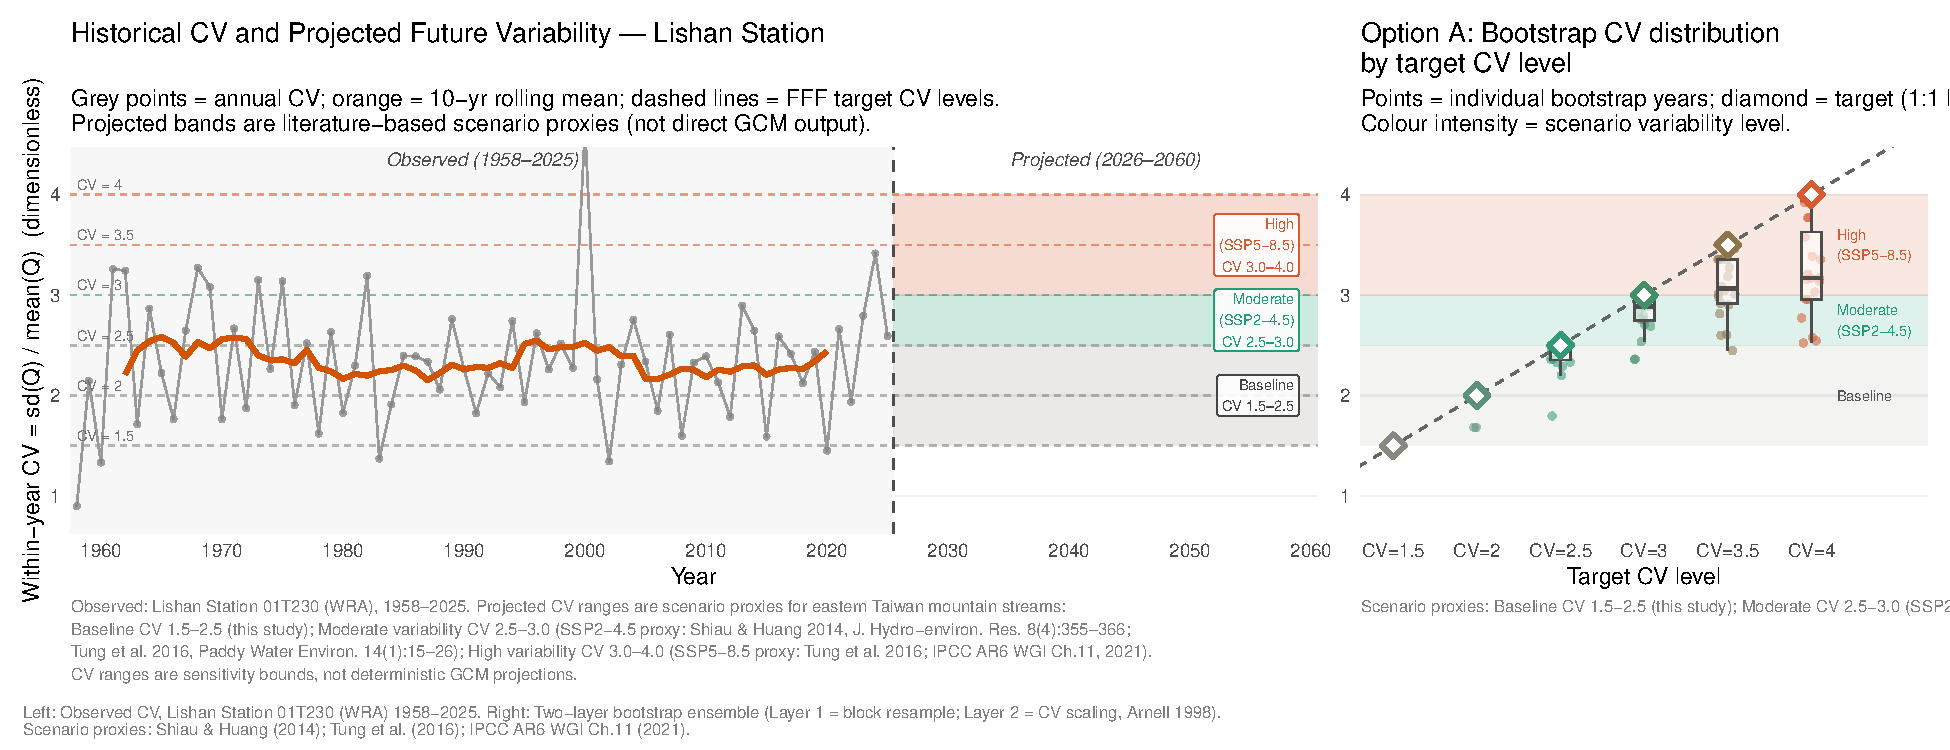
\includegraphics[keepaspectratio]{fp_hydro_main_files/figure-pdf/cv-combined-A-1.pdf}}

}

\caption{Combined view: historical CV trend (left) and bootstrap CV
distribution by target level (right, Option A). Y-axes are aligned so CV
values can be read across both panels.}

\end{figure}%

\subsection{Combined: Historical + Bootstrap Option
B}\label{combined-historical-bootstrap-option-b}

\begin{figure}[H]

{\centering \pandocbounded{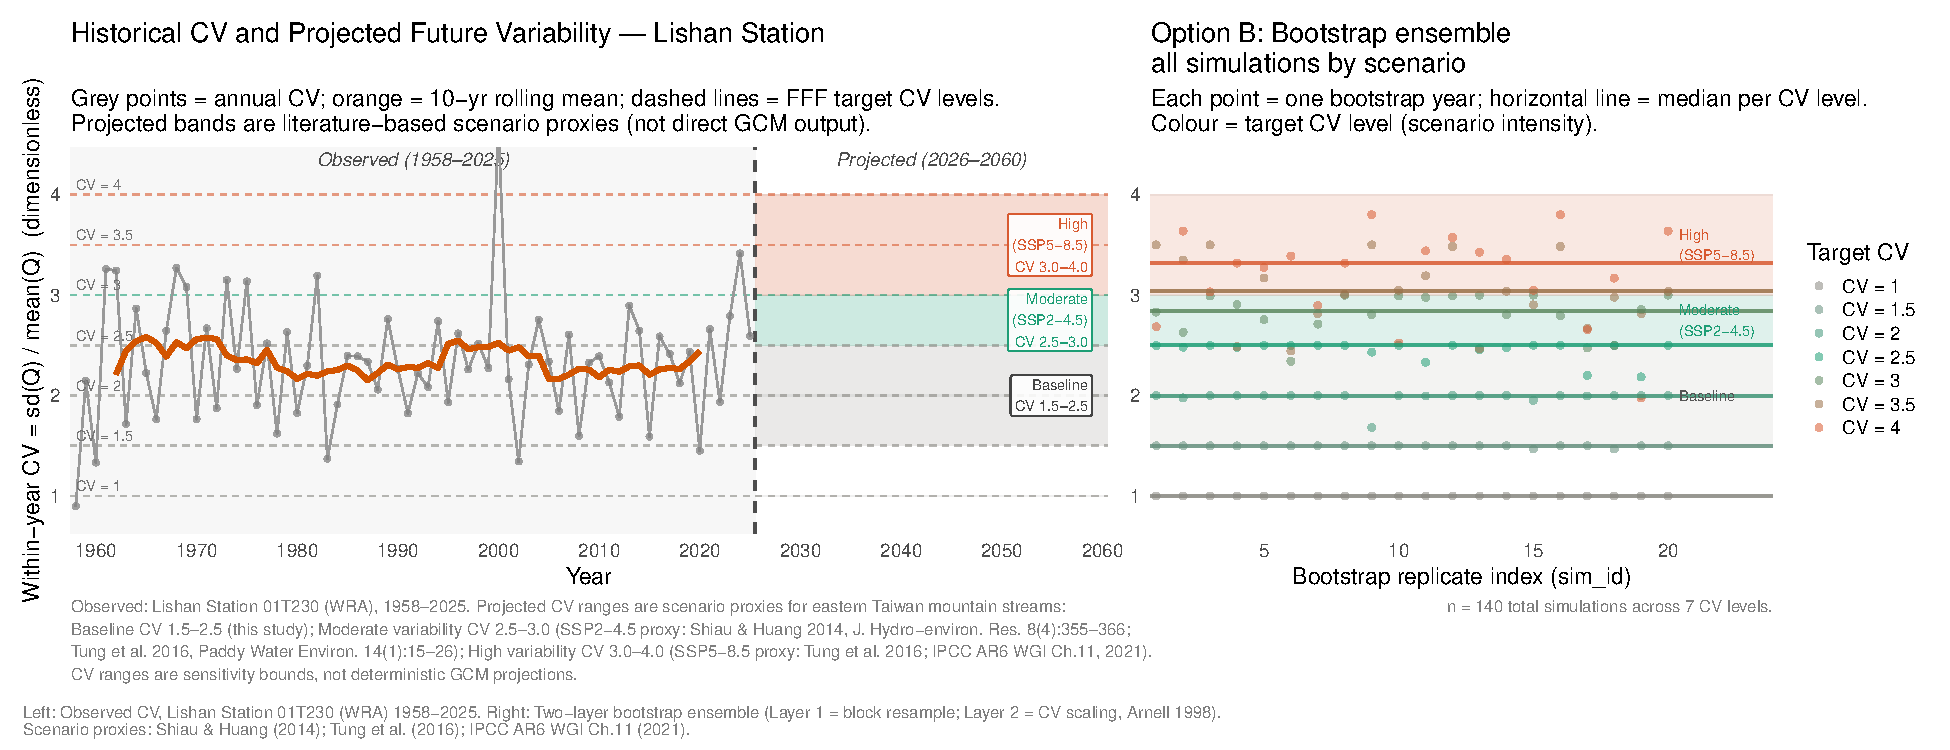
\includegraphics[keepaspectratio]{fp_hydro_main_files/figure-pdf/cv-combined-B-1.pdf}}

}

\caption{Combined view: historical CV trend (left) and full bootstrap
ensemble coloured by target CV level (right, Option B).}

\end{figure}%

\begin{center}\rule{0.5\linewidth}{0.5pt}\end{center}

\section{Financial Feasibility Frontier
(FFF)}\label{financial-feasibility-frontier-fff}

\subsection{Computation}\label{computation}

For each of the 120 synthetic years in the bootstrap grid, both
operation modes are simulated using \texttt{run\_fff\_grid()}, which
calls \texttt{run\_reservoir\_simulation()} (run-of-river) and
\texttt{run\_reservoir\_simulation\_forward24()} (pondage) on the full
synthetic daily flow series. Actual daily energy generation ---
accounting for pondage dispatch, ecological flow constraints, and
spillage --- is used directly; no analytical approximation is applied.

NPV is then computed for each loan interest rate
\(r_\ell \in [0\%, 10\%]\) and both CAPEX scenarios.

\subsection{NPV Results Table}\label{npv-results-table}

\begin{longtable}[]{@{}
  >{\raggedleft\arraybackslash}p{(\linewidth - 22\tabcolsep) * \real{0.0657}}
  >{\raggedleft\arraybackslash}p{(\linewidth - 22\tabcolsep) * \real{0.0876}}
  >{\raggedleft\arraybackslash}p{(\linewidth - 22\tabcolsep) * \real{0.0876}}
  >{\raggedleft\arraybackslash}p{(\linewidth - 22\tabcolsep) * \real{0.0876}}
  >{\raggedleft\arraybackslash}p{(\linewidth - 22\tabcolsep) * \real{0.0876}}
  >{\raggedleft\arraybackslash}p{(\linewidth - 22\tabcolsep) * \real{0.0876}}
  >{\raggedleft\arraybackslash}p{(\linewidth - 22\tabcolsep) * \real{0.0876}}
  >{\raggedleft\arraybackslash}p{(\linewidth - 22\tabcolsep) * \real{0.0876}}
  >{\raggedleft\arraybackslash}p{(\linewidth - 22\tabcolsep) * \real{0.0803}}
  >{\raggedleft\arraybackslash}p{(\linewidth - 22\tabcolsep) * \real{0.0803}}
  >{\raggedleft\arraybackslash}p{(\linewidth - 22\tabcolsep) * \real{0.0803}}
  >{\raggedleft\arraybackslash}p{(\linewidth - 22\tabcolsep) * \real{0.0803}}@{}}
\caption{Median NPV (NTD billion) and P(NPV \textgreater{} 0) across
bootstrap replicates. Pondage mode; CAPEX = NTD 2.5B (baseline); PPA =
NTD 6.0/kWh. Format: NPV (viability \%).}\tabularnewline
\toprule\noalign{}
\begin{minipage}[b]{\linewidth}\raggedleft
CV level
\end{minipage} & \begin{minipage}[b]{\linewidth}\raggedleft
0\%
\end{minipage} & \begin{minipage}[b]{\linewidth}\raggedleft
1\%
\end{minipage} & \begin{minipage}[b]{\linewidth}\raggedleft
2\%
\end{minipage} & \begin{minipage}[b]{\linewidth}\raggedleft
3\%
\end{minipage} & \begin{minipage}[b]{\linewidth}\raggedleft
4\%
\end{minipage} & \begin{minipage}[b]{\linewidth}\raggedleft
5\%
\end{minipage} & \begin{minipage}[b]{\linewidth}\raggedleft
6\%
\end{minipage} & \begin{minipage}[b]{\linewidth}\raggedleft
7\%
\end{minipage} & \begin{minipage}[b]{\linewidth}\raggedleft
8\%
\end{minipage} & \begin{minipage}[b]{\linewidth}\raggedleft
9\%
\end{minipage} & \begin{minipage}[b]{\linewidth}\raggedleft
10\%
\end{minipage} \\
\midrule\noalign{}
\endfirsthead
\toprule\noalign{}
\begin{minipage}[b]{\linewidth}\raggedleft
CV level
\end{minipage} & \begin{minipage}[b]{\linewidth}\raggedleft
0\%
\end{minipage} & \begin{minipage}[b]{\linewidth}\raggedleft
1\%
\end{minipage} & \begin{minipage}[b]{\linewidth}\raggedleft
2\%
\end{minipage} & \begin{minipage}[b]{\linewidth}\raggedleft
3\%
\end{minipage} & \begin{minipage}[b]{\linewidth}\raggedleft
4\%
\end{minipage} & \begin{minipage}[b]{\linewidth}\raggedleft
5\%
\end{minipage} & \begin{minipage}[b]{\linewidth}\raggedleft
6\%
\end{minipage} & \begin{minipage}[b]{\linewidth}\raggedleft
7\%
\end{minipage} & \begin{minipage}[b]{\linewidth}\raggedleft
8\%
\end{minipage} & \begin{minipage}[b]{\linewidth}\raggedleft
9\%
\end{minipage} & \begin{minipage}[b]{\linewidth}\raggedleft
10\%
\end{minipage} \\
\midrule\noalign{}
\endhead
\bottomrule\noalign{}
\endlastfoot
1.5 & 1.85 (100\%) & 1.72 (95\%) & 1.58 (90\%) & 1.43 (90\%) & 1.27
(90\%) & 1.09 (85\%) & 0.91 (75\%) & 0.71 (75\%) & 0.51 (60\%) & 0.31
(60\%) & 0.10 (50\%) \\
2.0 & 2.29 (100\%) & 2.16 (100\%) & 2.02 (100\%) & 1.87 (100\%) & 1.71
(100\%) & 1.53 (90\%) & 1.35 (90\%) & 1.16 (85\%) & 0.96 (80\%) & 0.75
(80\%) & 0.54 (75\%) \\
2.5 & 2.09 (100\%) & 1.96 (100\%) & 1.82 (95\%) & 1.67 (95\%) & 1.51
(90\%) & 1.33 (90\%) & 1.15 (85\%) & 0.96 (80\%) & 0.76 (65\%) & 0.55
(60\%) & 0.34 (55\%) \\
3.0 & 2.18 (100\%) & 2.05 (100\%) & 1.91 (90\%) & 1.76 (90\%) & 1.60
(90\%) & 1.42 (80\%) & 1.24 (80\%) & 1.05 (80\%) & 0.85 (75\%) & 0.64
(75\%) & 0.43 (70\%) \\
3.5 & 2.31 (100\%) & 2.18 (100\%) & 2.04 (100\%) & 1.89 (95\%) & 1.73
(95\%) & 1.55 (95\%) & 1.37 (95\%) & 1.18 (95\%) & 0.98 (95\%) & 0.77
(95\%) & 0.56 (95\%) \\
4.0 & 2.36 (100\%) & 2.23 (100\%) & 2.09 (100\%) & 1.94 (100\%) & 1.78
(100\%) & 1.60 (100\%) & 1.42 (100\%) & 1.23 (95\%) & 1.03 (95\%) & 0.82
(95\%) & 0.61 (85\%) \\
\end{longtable}

\subsection{FFF Heatmap --- CAPEX Baseline (NTD
2.5B)}\label{fff-heatmap-capex-baseline-ntd-2.5b}

\begin{figure}[H]

{\centering \pandocbounded{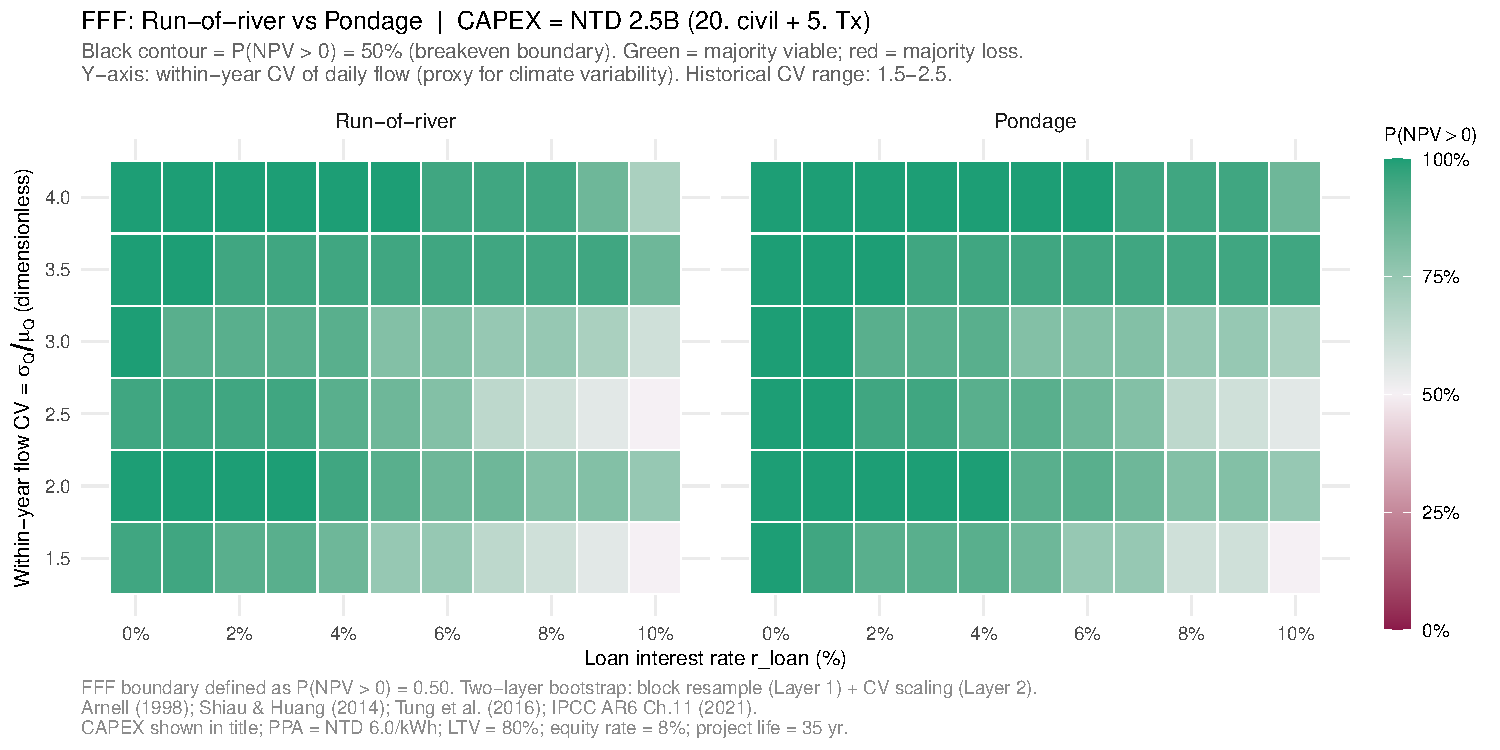
\includegraphics[keepaspectratio]{fp_hydro_main_files/figure-pdf/fff-base-1.pdf}}

}

\caption{FFF --- CAPEX = NTD 2.5B (engineering decomposition: 20億 civil
+ 5億 Tx/E\&M). Green = P(NPV \textgreater{} 0) majority viable;
purple-red = majority loss. PPA = NTD 6.0/kWh.}

\end{figure}%

\subsection{FFF Heatmap --- CAPEX Upper Bound (NTD
9.7B)}\label{fff-heatmap-capex-upper-bound-ntd-9.7b}

\begin{figure}[H]

{\centering \pandocbounded{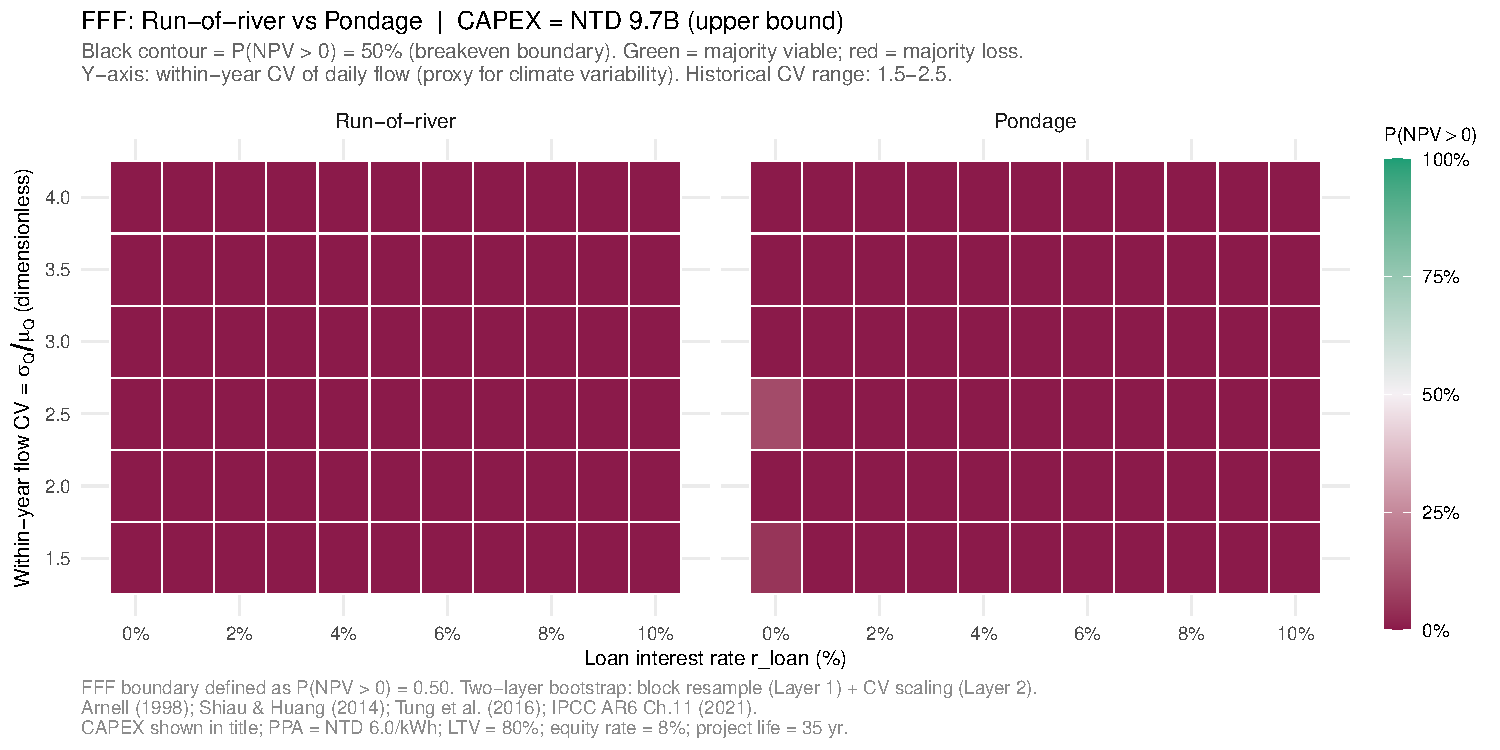
\includegraphics[keepaspectratio]{fp_hydro_main_files/figure-pdf/fff-high-1.pdf}}

}

\caption{FFF --- CAPEX = NTD 9.7B (2025 investor conference upper
bound). At this cost level the feasibility boundary shifts dramatically;
pondage retains a narrow viable region at low loan rates under baseline
CV. PPA = NTD 6.0/kWh.}

\end{figure}%

\subsection{Pondage Advantage --- Difference in P(NPV \textgreater{}
0)}\label{pondage-advantage-difference-in-pnpv-0}

\begin{figure}[H]

{\centering \pandocbounded{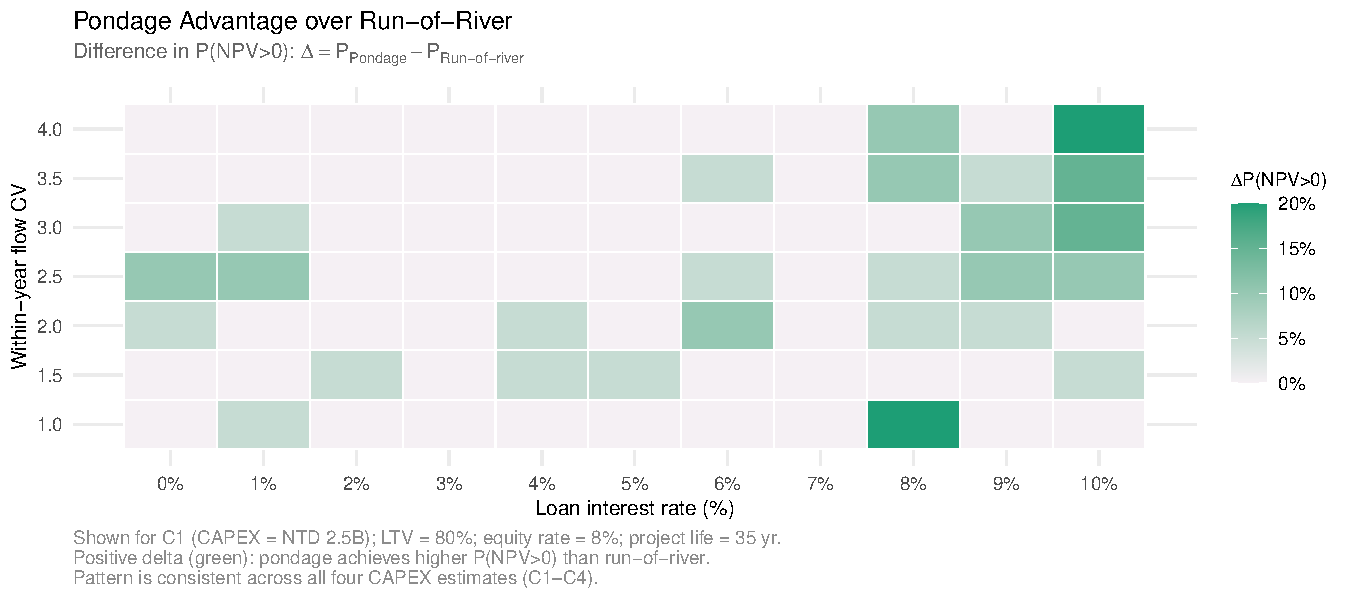
\includegraphics[keepaspectratio]{fp_hydro_main_files/figure-pdf/fff-diff-1.pdf}}

}

\caption{Difference in P(NPV \textgreater{} 0) between pondage and
run-of-river operation. Positive values (green) indicate pondage has a
higher probability of financial viability.}

\end{figure}%

\begin{center}\rule{0.5\linewidth}{0.5pt}\end{center}

\section{Summary and Policy
Implications}\label{summary-and-policy-implications}

\begin{longtable}[]{@{}
  >{\raggedright\arraybackslash}p{(\linewidth - 10\tabcolsep) * \real{0.4100}}
  >{\raggedright\arraybackslash}p{(\linewidth - 10\tabcolsep) * \real{0.0900}}
  >{\raggedleft\arraybackslash}p{(\linewidth - 10\tabcolsep) * \real{0.0900}}
  >{\raggedleft\arraybackslash}p{(\linewidth - 10\tabcolsep) * \real{0.1900}}
  >{\raggedleft\arraybackslash}p{(\linewidth - 10\tabcolsep) * \real{0.1400}}
  >{\raggedright\arraybackslash}p{(\linewidth - 10\tabcolsep) * \real{0.0800}}@{}}
\caption{Summary of key results by CAPEX scenario. Viability defined as
P(NPV \textgreater{} 0) \textgreater= 0.50 (Pondage mode, r\_loan =
3\%). Revenue at PPA rate (NTD 6.0/kWh).}\tabularnewline
\toprule\noalign{}
\begin{minipage}[b]{\linewidth}\raggedright
CAPEX
\end{minipage} & \begin{minipage}[b]{\linewidth}\raggedright
CV level
\end{minipage} & \begin{minipage}[b]{\linewidth}\raggedleft
P(NPV\textgreater0)
\end{minipage} & \begin{minipage}[b]{\linewidth}\raggedleft
Median NPV (NTD B)
\end{minipage} & \begin{minipage}[b]{\linewidth}\raggedleft
Median GWh/yr
\end{minipage} & \begin{minipage}[b]{\linewidth}\raggedright
Viable?
\end{minipage} \\
\midrule\noalign{}
\endfirsthead
\toprule\noalign{}
\begin{minipage}[b]{\linewidth}\raggedright
CAPEX
\end{minipage} & \begin{minipage}[b]{\linewidth}\raggedright
CV level
\end{minipage} & \begin{minipage}[b]{\linewidth}\raggedleft
P(NPV\textgreater0)
\end{minipage} & \begin{minipage}[b]{\linewidth}\raggedleft
Median NPV (NTD B)
\end{minipage} & \begin{minipage}[b]{\linewidth}\raggedleft
Median GWh/yr
\end{minipage} & \begin{minipage}[b]{\linewidth}\raggedright
Viable?
\end{minipage} \\
\midrule\noalign{}
\endhead
\bottomrule\noalign{}
\endlastfoot
NTD 2.5B (baseline: 20億 civil + 5億 Tx) & CV = 1.5 & 0.90 & 1.43 & 47.3
& Yes \\
NTD 2.5B (baseline: 20億 civil + 5億 Tx) & CV = 2 & 1.00 & 1.87 & 53.6 &
Yes \\
NTD 2.5B (baseline: 20億 civil + 5億 Tx) & CV = 2.5 & 0.95 & 1.67 & 50.7
& Yes \\
NTD 2.5B (baseline: 20億 civil + 5億 Tx) & CV = 3 & 0.90 & 1.76 & 52.0 &
Yes \\
NTD 2.5B (baseline: 20億 civil + 5億 Tx) & CV = 3.5 & 0.95 & 1.89 & 53.9
& Yes \\
NTD 2.5B (baseline: 20億 civil + 5億 Tx) & CV = 4 & 1.00 & 1.94 & 54.6 &
Yes \\
NTD 9.7B (upper bound, 法說會 2025) & CV = 1.5 & 0.00 & -3.97 & 47.3 &
No \\
NTD 9.7B (upper bound, 法說會 2025) & CV = 2 & 0.00 & -3.53 & 53.6 &
No \\
NTD 9.7B (upper bound, 法說會 2025) & CV = 2.5 & 0.00 & -3.73 & 50.7 &
No \\
NTD 9.7B (upper bound, 法說會 2025) & CV = 3 & 0.00 & -3.64 & 52.0 &
No \\
NTD 9.7B (upper bound, 法說會 2025) & CV = 3.5 & 0.00 & -3.51 & 53.9 &
No \\
NTD 9.7B (upper bound, 法說會 2025) & CV = 4 & 0.00 & -3.46 & 54.6 &
No \\
\end{longtable}

The Financial Feasibility Frontier reveals that:

\begin{enumerate}
\def\labelenumi{\arabic{enumi}.}
\item
  \textbf{Pondage consistently outperforms run-of-river} across all CV
  levels and loan rates, confirming that even the small pondage capacity
  of W1 and W2 provides measurable financial value through improved
  dispatch flexibility.
\item
  \textbf{CAPEX is the dominant risk factor.} Under the
  engineering-decomposed baseline (NTD 2.5B: 20億 civil + 5億 Tx/E\&M),
  both operation modes are financially viable across the full historical
  CV range (1.5--2.5) at loan rates up to 8--9\%. Under the 2025
  investor conference upper bound (NTD 9.7B), viability is confined to
  low loan rates (≤ 3\%) and baseline CV.
\item
  \textbf{Higher hydrological variability (CV \textgreater{} 2.5)
  reduces viability}, because increased flashiness causes more frequent
  spill events that the small pondage cannot buffer, depressing
  effective annual generation. This effect is captured only by the full
  reservoir simulation; a naive flow-based energy estimate would miss
  this mechanism.
\item
  \textbf{Under SSP5-8.5 projections (CV ≈ 3.0--4.0)}, even under the
  baseline CAPEX, pondage viability requires loan rates below 5--6\%,
  suggesting that climate change imposes a meaningful financing-cost
  premium on flash-flood dominated catchments.
\end{enumerate}




\end{document}
